\documentclass[../AnalysisNoteJBuxton.tex]{subfiles}
\begin{document}

\subsection{Stavinsky Correlation Function Construction}
\label{StavCfConstruction}

Stavinsky is tight.


\begin{figure}[h!]
  \centering
  %%----start of first subfigure---  
  \subfloat[\LamKchP (left) and \ALamKchM (right) correlations for 0-10\% (top), 10-30\%(middle), and 30-50\%(bottom) centralities.]{
    \label{fig:StavCfs:a}
    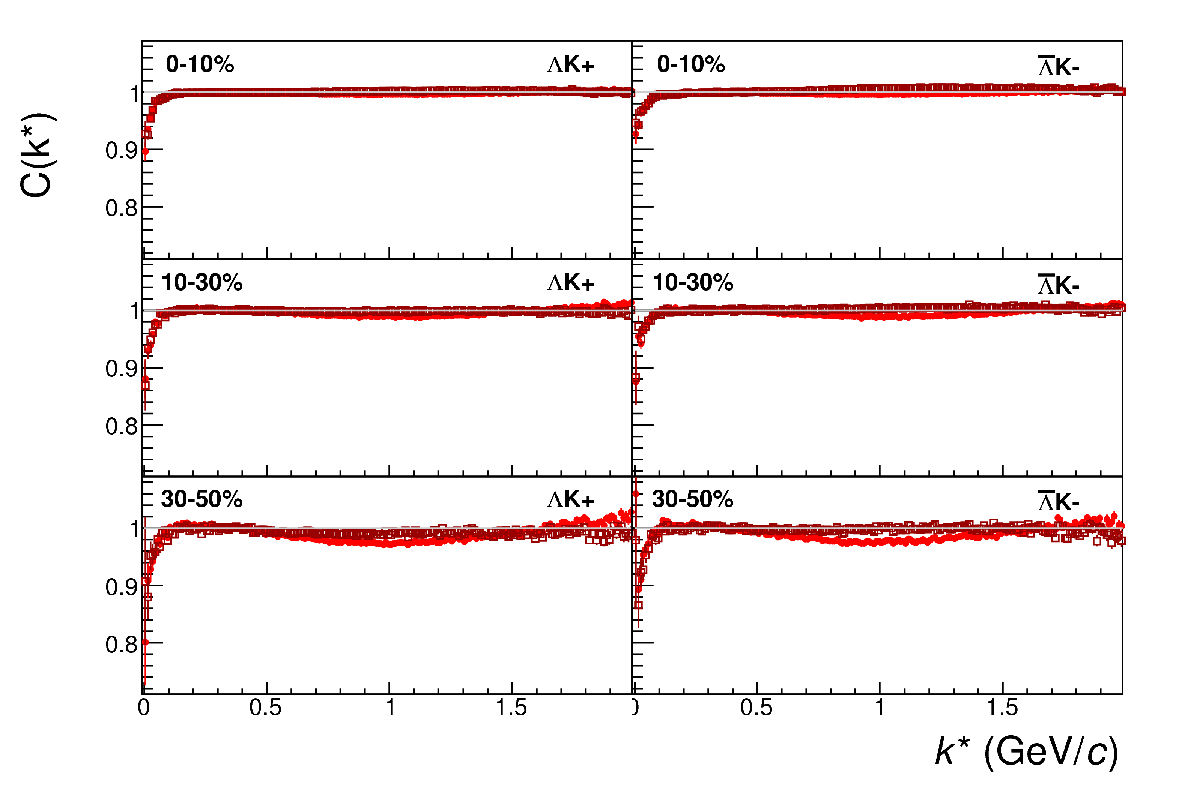
\includegraphics[width=0.49\textwidth]{4_CorrelationFunctions/Figures/WithAdditionalPairCut_20180505/canKStarCfsLamKchPwConj_20180505vs20180505StavCf.pdf}}
  %%----start of second subfigure---
  \subfloat[\LamKchM (left) and \ALamKchP (right) correlations for 0-10\% (top), 10-30\%(middle), and 30-50\%(bottom) centralities.]{
    \label{fig:StavCfs:b}
    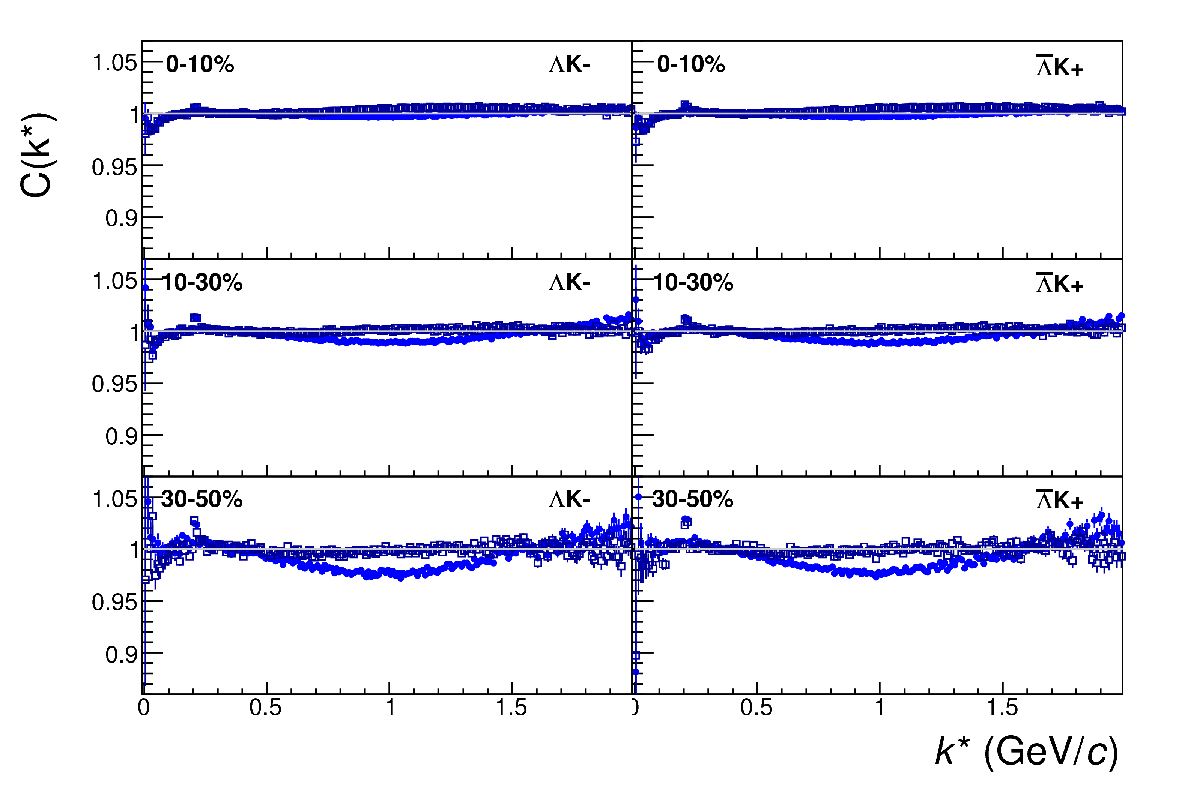
\includegraphics[width=0.49\textwidth]{4_CorrelationFunctions/Figures/WithAdditionalPairCut_20180505/canKStarCfsLamKchMwConj_20180505vs20180505StavCf.pdf}}
  \\  
  %%----start of third subfigure---
  \subfloat[\LamKs (left) and \ALamKs (right) correlations for 0-10\% (top), 10-30\%(middle), and 30-50\%(bottom) centralities.]{
    \label{fig:StavCfs:c}
    \includegraphics[width=0.49\textwidth]{4_CorrelationFunctions/Figures/WithAdditionalPairCut_20180505/canKStarCfsLamK0wConj_20180505vs20180505StavCf.pdf}}    
  %%----overall caption----
  \caption[\LamK Stavinsky Correlation Functions]{\LamK and \ALamAK correlation functions built using the Stavinsky method for 0-10\%, 10-30\%, and 30-50\% centralities.}
  \label{fig:StavCfs}
\end{figure}


\begin{figure}[h!]
  \centering
  %%----start of first subfigure---  
  \subfloat[\LamKchP (left) and \ALamKchM (right) correlations for 0-10\% (top), 10-30\%(middle), and 30-50\%(bottom) centralities.]{
    \label{fig:AllStavCfs_Zoom:a}
    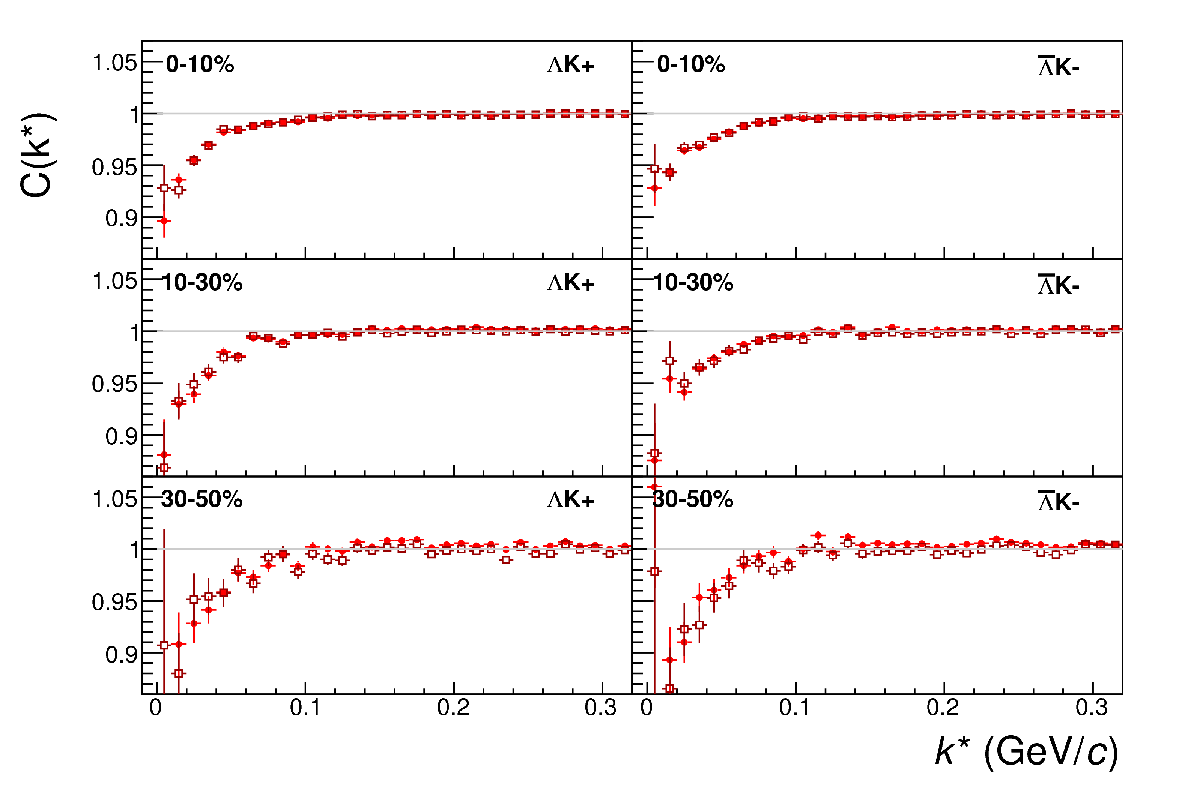
\includegraphics[width=0.49\textwidth]{4_CorrelationFunctions/Figures/WithAdditionalPairCut_20180505/canKStarCfsZoomLamKchPwConj_20180505vs20180505StavCf.pdf}}
  %%----start of second subfigure---
  \subfloat[\LamKchM (left) and \ALamKchP (right) correlations for 0-10\% (top), 10-30\%(middle), and 30-50\%(bottom) centralities.]{
    \label{fig:AllStavCfs_Zoom:b}
    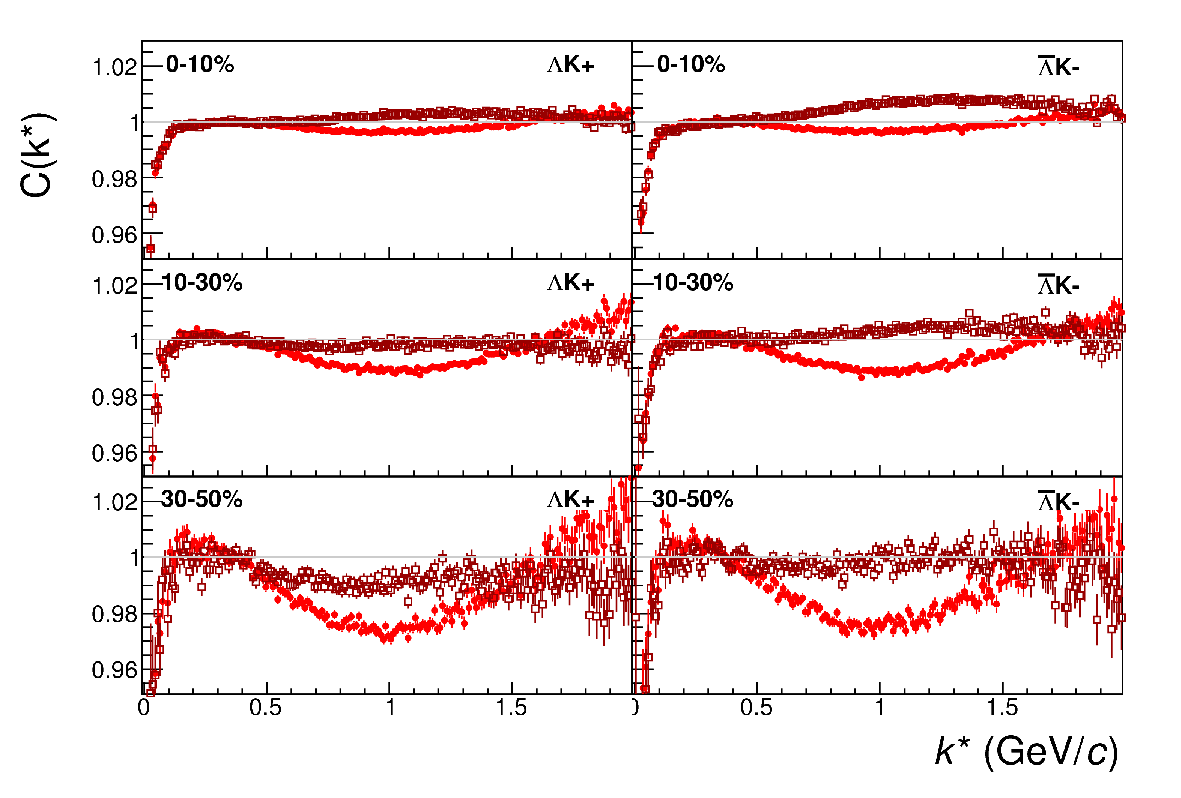
\includegraphics[width=0.49\textwidth]{4_CorrelationFunctions/Figures/WithAdditionalPairCut_20180505/canKStarCfsZoomYAxisLamKchPwConj_20180505vs20180505StavCf.pdf}}
  \\  
  
  %%----start of third subfigure---  
  \subfloat[\LamKchP (left) and \ALamKchM (right) correlations for 0-10\% (top), 10-30\%(middle), and 30-50\%(bottom) centralities.]{
    \label{fig:AllStavCfs_Zoom:a}
    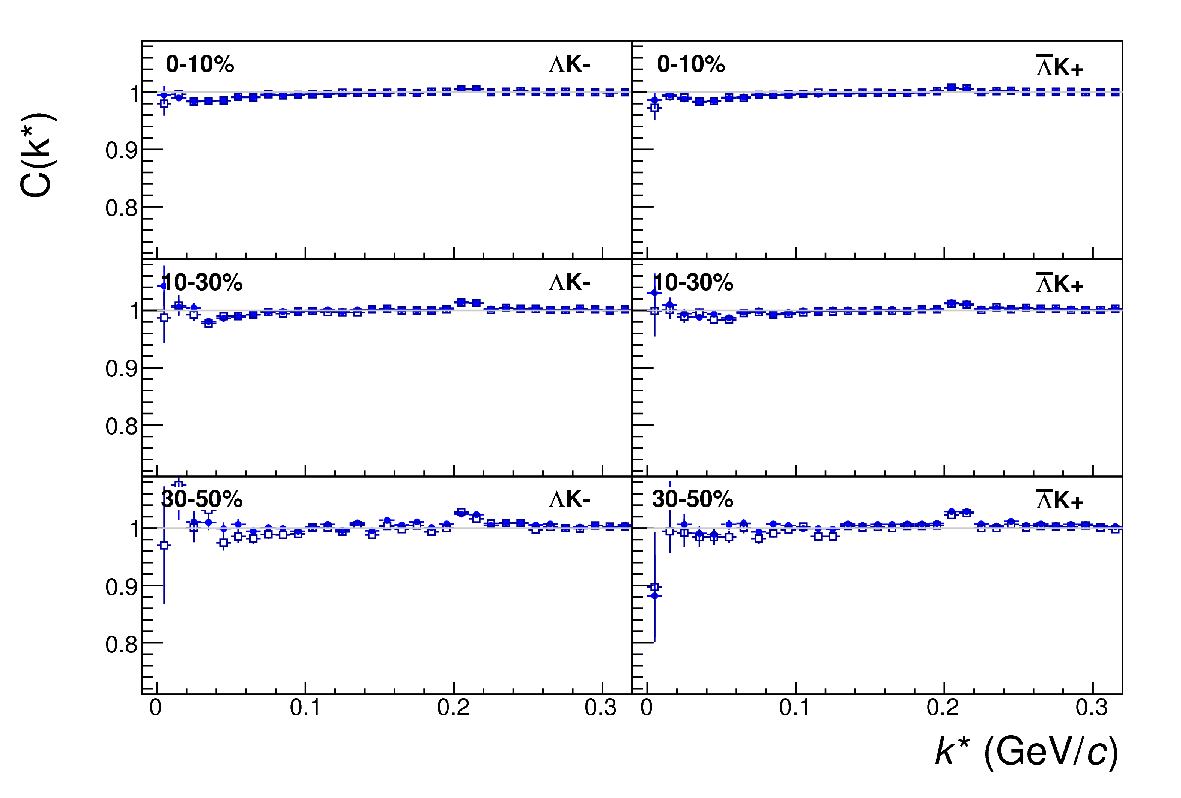
\includegraphics[width=0.49\textwidth]{4_CorrelationFunctions/Figures/WithAdditionalPairCut_20180505/canKStarCfsZoomLamKchMwConj_20180505vs20180505StavCf.pdf}}
  %%----start of fourth subfigure---
  \subfloat[\LamKchM (left) and \ALamKchP (right) correlations for 0-10\% (top), 10-30\%(middle), and 30-50\%(bottom) centralities.]{
    \label{fig:AllStavCfs_Zoom:b}
    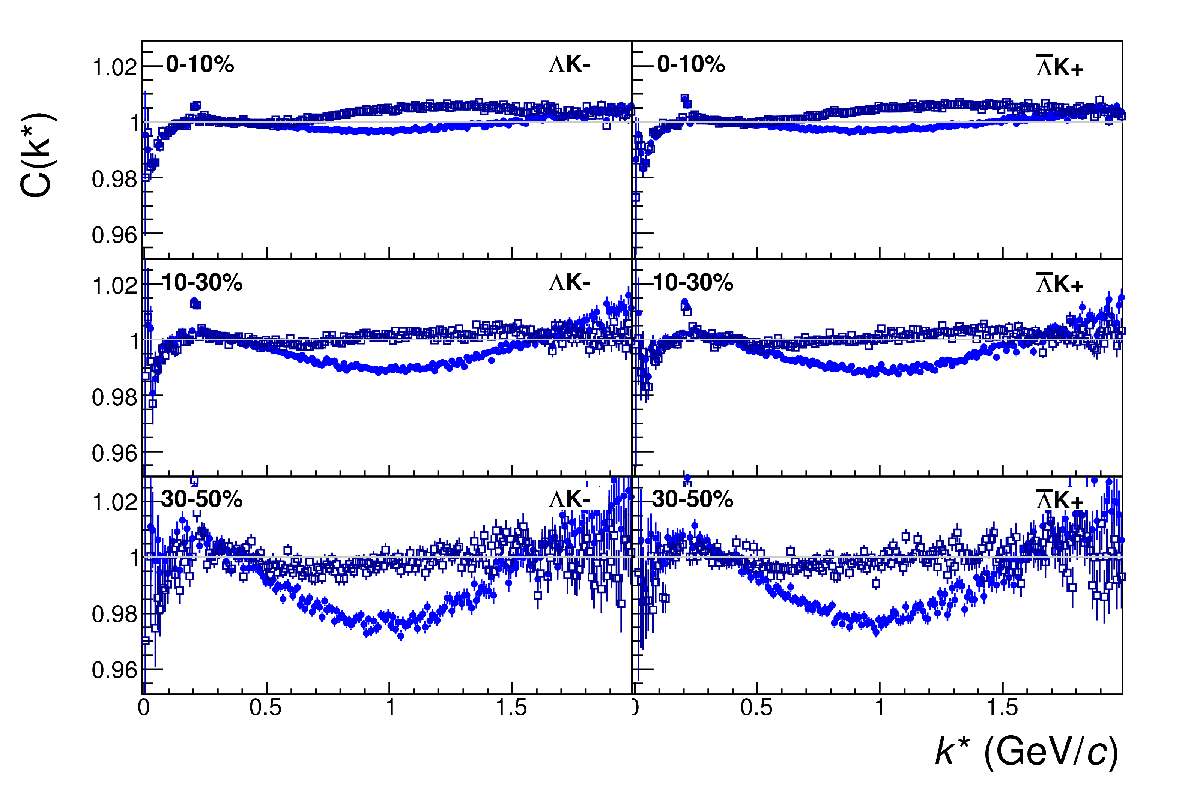
\includegraphics[width=0.49\textwidth]{4_CorrelationFunctions/Figures/WithAdditionalPairCut_20180505/canKStarCfsZoomYAxisLamKchMwConj_20180505vs20180505StavCf.pdf}}
  \\  
    
  %%----start of fifth subfigure---  
  \subfloat[\LamKchP (left) and \ALamKchM (right) correlations for 0-10\% (top), 10-30\%(middle), and 30-50\%(bottom) centralities.]{
    \label{fig:AllStavCfs_Zoom:a}
    \includegraphics[width=0.49\textwidth]{4_CorrelationFunctions/Figures/WithAdditionalPairCut_20180505/canKStarCfsZoomLamK0wConj_20180505vs20180505StavCf.pdf}}
  %%----start of sixth subfigure---
  \subfloat[\LamKchM (left) and \ALamKchP (right) correlations for 0-10\% (top), 10-30\%(middle), and 30-50\%(bottom) centralities.]{
    \label{fig:AllStavCfs_Zoom:b}
    \includegraphics[width=0.49\textwidth]{4_CorrelationFunctions/Figures/WithAdditionalPairCut_20180505/canKStarCfsZoomYAxisLamK0wConj_20180505vs20180505StavCf.pdf}}
  \\      
    
    
  %%----overall caption----
  \caption[\LamK Stavinsky Correlation Functions]{\LamK and \ALamAK correlation functions built using the Stavinsky method for 0-10\%, 10-30\%, and 30-50\% centralities.}
  \label{fig:AllStavCfs_Zoom}
\end{figure}









\begin{figure}[h!]
  \centering
  %%----start of first subfigure---  
  \subfloat[\LamKchP (left) and \ALamKchM (right) correlations for 0-10\% (top), 10-30\%(middle), and 30-50\%(bottom) centralities.]{
    \label{fig:AllStavCfs:a}
    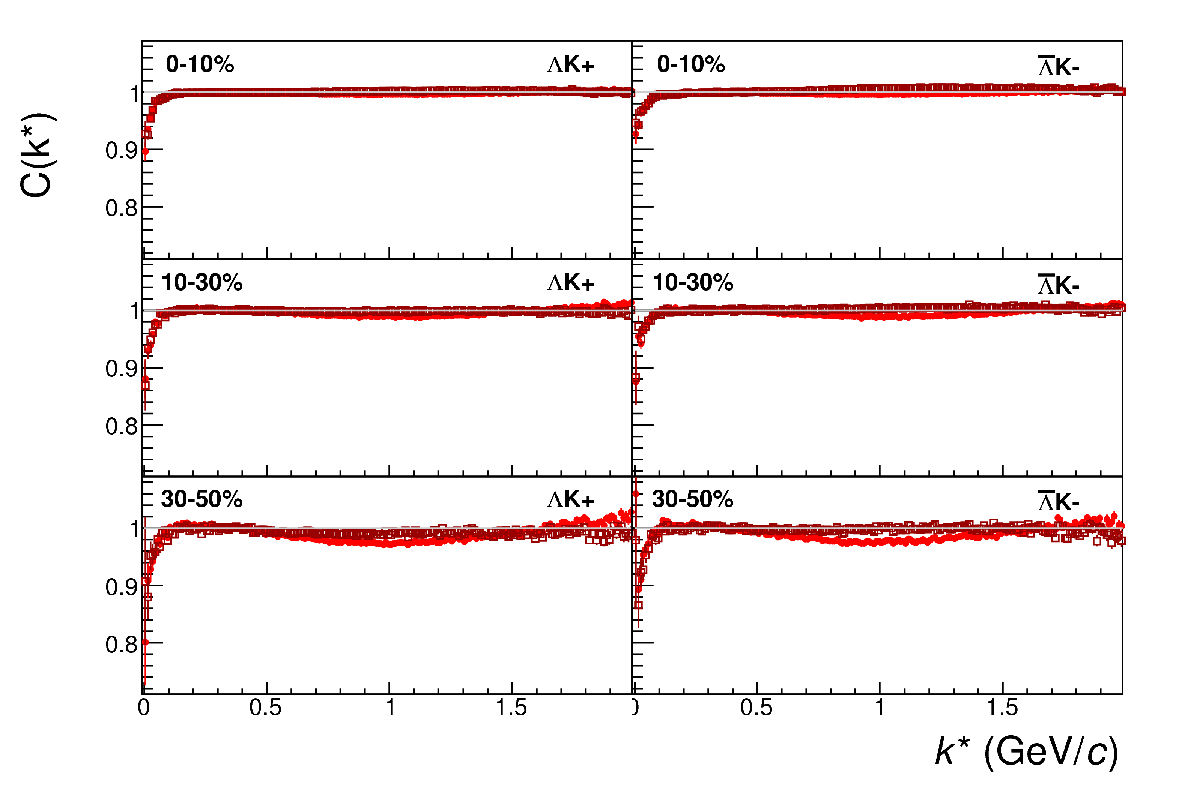
\includegraphics[width=0.49\textwidth]{4_CorrelationFunctions/Figures/WithAdditionalPairCut_20180505/canKStarCfsLamKchPwConj_20180505vs20180505StavCf.pdf}}
  %%----start of second subfigure---
  \subfloat[\LamKchM (left) and \ALamKchP (right) correlations for 0-10\% (top), 10-30\%(middle), and 30-50\%(bottom) centralities.]{
    \label{fig:AllStavCfs:b}
    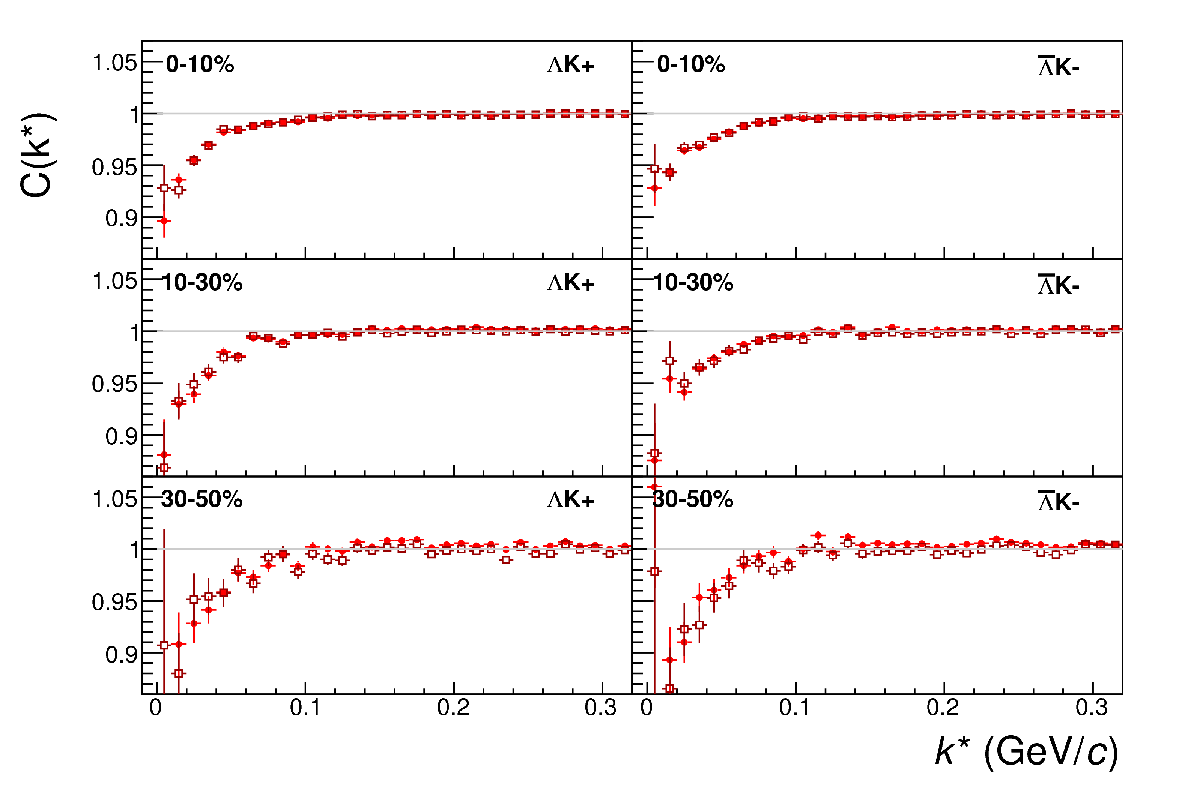
\includegraphics[width=0.49\textwidth]{4_CorrelationFunctions/Figures/WithAdditionalPairCut_20180505/canKStarCfsZoomLamKchPwConj_20180505vs20180505StavCf.pdf}}
  \\    
  
  %%----start of third subfigure---  
  \subfloat[\LamKchP (left) and \ALamKchM (right) correlations for 0-10\% (top), 10-30\%(middle), and 30-50\%(bottom) centralities.]{
    \label{fig:AllStavCfs:a}
    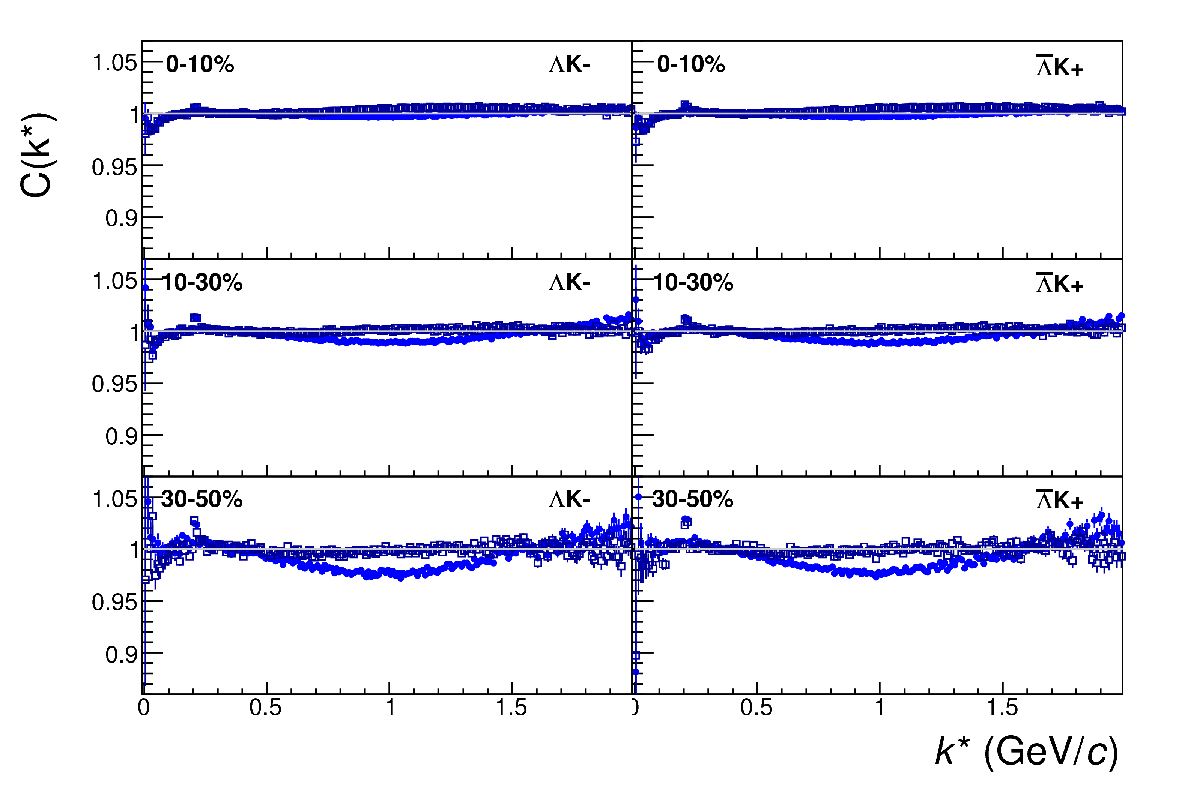
\includegraphics[width=0.49\textwidth]{4_CorrelationFunctions/Figures/WithAdditionalPairCut_20180505/canKStarCfsLamKchMwConj_20180505vs20180505StavCf.pdf}}
  %%----start of fourth subfigure---
  \subfloat[\LamKchM (left) and \ALamKchP (right) correlations for 0-10\% (top), 10-30\%(middle), and 30-50\%(bottom) centralities.]{
    \label{fig:AllStavCfs:b}
    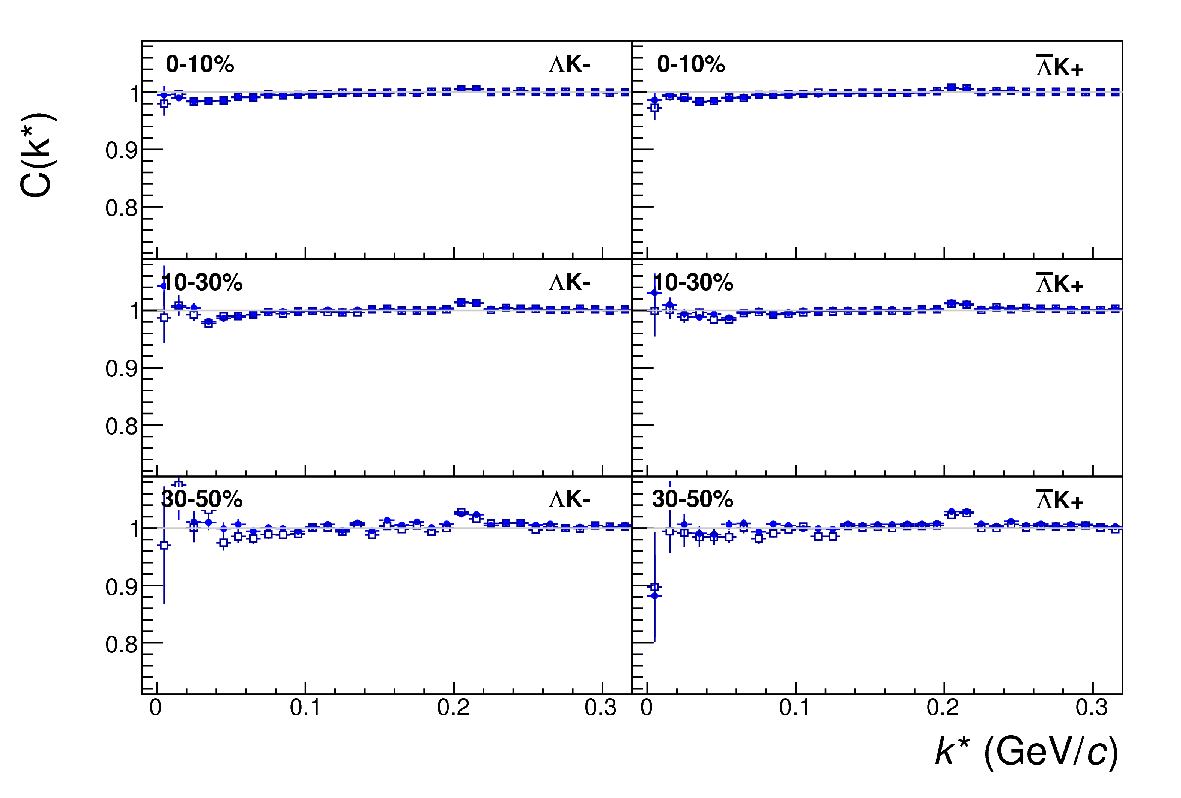
\includegraphics[width=0.49\textwidth]{4_CorrelationFunctions/Figures/WithAdditionalPairCut_20180505/canKStarCfsZoomLamKchMwConj_20180505vs20180505StavCf.pdf}}
  \\    
    
  %%----start of fifth subfigure---  
  \subfloat[\LamKchP (left) and \ALamKchM (right) correlations for 0-10\% (top), 10-30\%(middle), and 30-50\%(bottom) centralities.]{
    \label{fig:AllStavCfs:a}
    \includegraphics[width=0.49\textwidth]{4_CorrelationFunctions/Figures/WithAdditionalPairCut_20180505/canKStarCfsLamK0wConj_20180505vs20180505StavCf.pdf}}
  %%----start of sixth subfigure---
  \subfloat[\LamKchM (left) and \ALamKchP (right) correlations for 0-10\% (top), 10-30\%(middle), and 30-50\%(bottom) centralities.]{
    \label{fig:AllStavCfs:b}
    \includegraphics[width=0.49\textwidth]{4_CorrelationFunctions/Figures/WithAdditionalPairCut_20180505/canKStarCfsZoomLamK0wConj_20180505vs20180505StavCf.pdf}}
  \\         
    
  %%----overall caption----
  \caption[\LamK Stavinsky Correlation Functions]{\LamK and \ALamAK correlation functions built using the Stavinsky method for 0-10\%, 10-30\%, and 30-50\% centralities.}
  \label{fig:AllStavCfs}
\end{figure}











\begin{figure}[h!]
  \centering
  %%----start of first subfigure---  
  \subfloat[\LamKchP (left) and \ALamKchM (right) correlations for 0-10\% (top), 10-30\%(middle), and 30-50\%(bottom) centralities.]{
    \label{fig:AllStavCfs:a}
    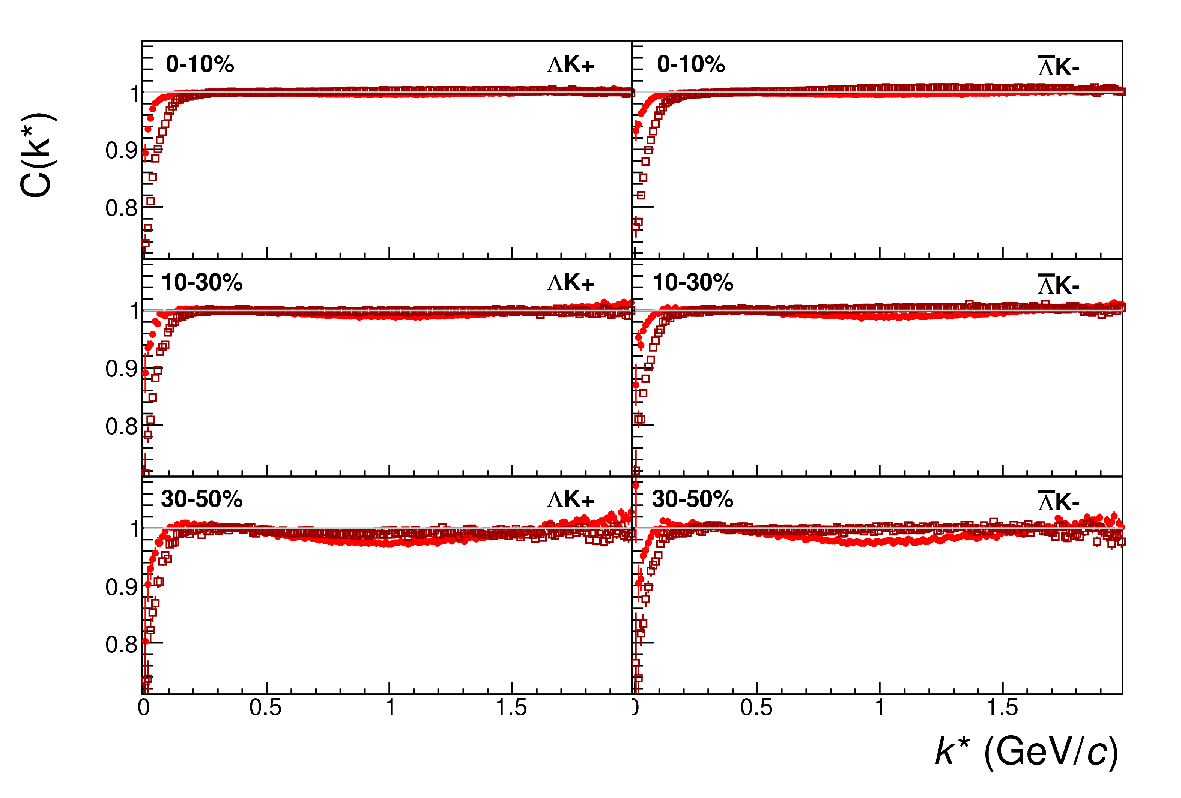
\includegraphics[width=0.49\textwidth]{4_CorrelationFunctions/Figures/WithoutAdditionalPairCut_20180416/canKStarCfsLamKchPwConj_20180416vs20180416StavCf.pdf}}
  %%----start of second subfigure---
  \subfloat[\LamKchM (left) and \ALamKchP (right) correlations for 0-10\% (top), 10-30\%(middle), and 30-50\%(bottom) centralities.]{
    \label{fig:AllStavCfs:b}
    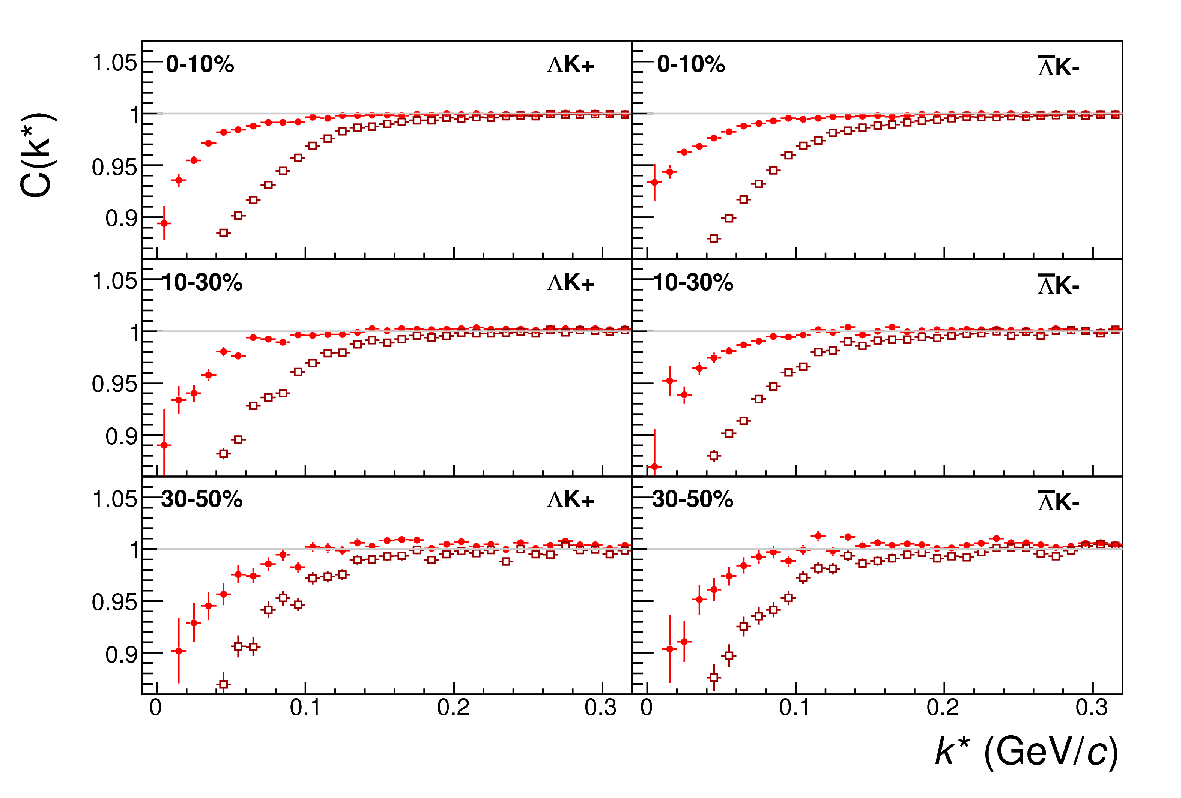
\includegraphics[width=0.49\textwidth]{4_CorrelationFunctions/Figures/WithoutAdditionalPairCut_20180416/canKStarCfsZoomLamKchPwConj_20180416vs20180416StavCf.pdf}}
  \\    
  
  %%----start of third subfigure---  
  \subfloat[\LamKchP (left) and \ALamKchM (right) correlations for 0-10\% (top), 10-30\%(middle), and 30-50\%(bottom) centralities.]{
    \label{fig:AllStavCfs:a}
    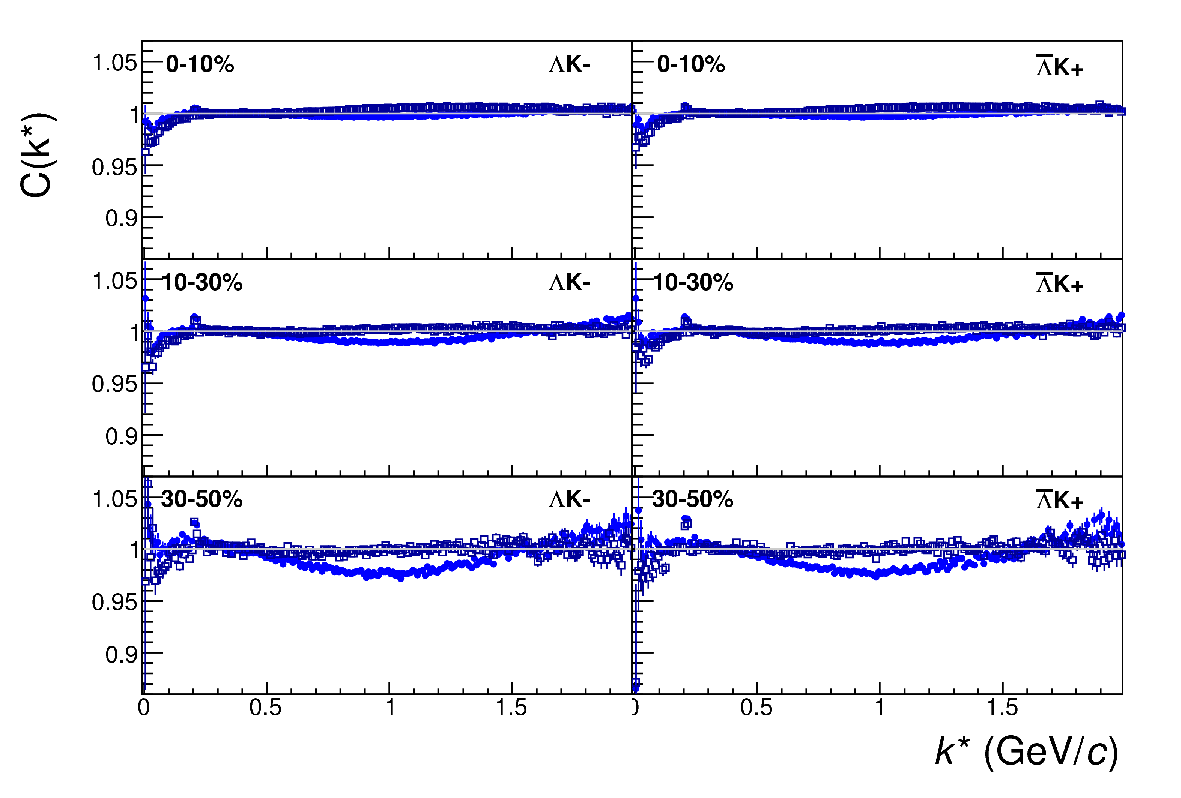
\includegraphics[width=0.49\textwidth]{4_CorrelationFunctions/Figures/WithoutAdditionalPairCut_20180416/canKStarCfsLamKchMwConj_20180416vs20180416StavCf.pdf}}
  %%----start of fourth subfigure---
  \subfloat[\LamKchM (left) and \ALamKchP (right) correlations for 0-10\% (top), 10-30\%(middle), and 30-50\%(bottom) centralities.]{
    \label{fig:AllStavCfs:b}
    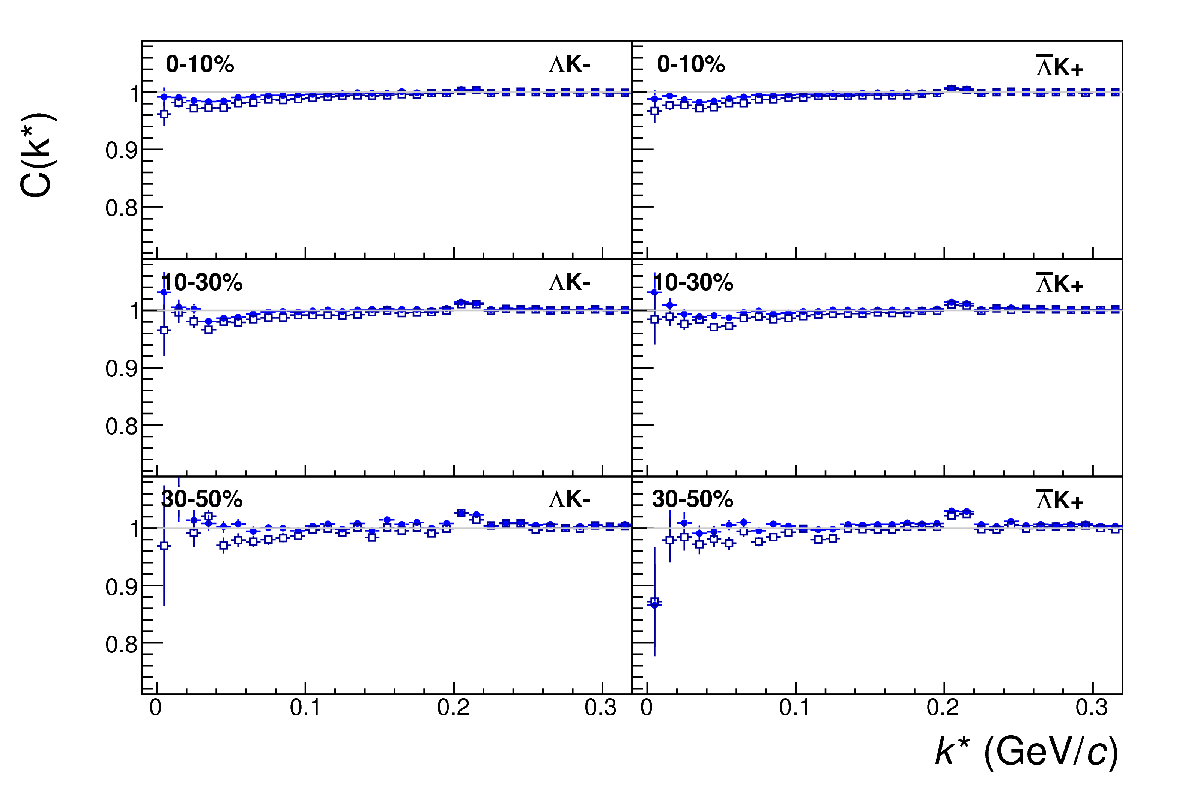
\includegraphics[width=0.49\textwidth]{4_CorrelationFunctions/Figures/WithoutAdditionalPairCut_20180416/canKStarCfsZoomLamKchMwConj_20180416vs20180416StavCf.pdf}}
  \\    
    
  %%----start of fifth subfigure---  
  \subfloat[\LamKchP (left) and \ALamKchM (right) correlations for 0-10\% (top), 10-30\%(middle), and 30-50\%(bottom) centralities.]{
    \label{fig:AllStavCfs:a}
    \includegraphics[width=0.49\textwidth]{4_CorrelationFunctions/Figures/WithoutAdditionalPairCut_20180416/canKStarCfsLamK0wConj_20180416vs20180416StavCf.pdf}}
  %%----start of sixth subfigure---
  \subfloat[\LamKchM (left) and \ALamKchP (right) correlations for 0-10\% (top), 10-30\%(middle), and 30-50\%(bottom) centralities.]{
    \label{fig:AllStavCfs:b}
    \includegraphics[width=0.49\textwidth]{4_CorrelationFunctions/Figures/WithoutAdditionalPairCut_20180416/canKStarCfsZoomLamK0wConj_20180416vs20180416StavCf.pdf}}
  \\         
    
  %%----overall caption----
  \caption[\LamK Stavinsky Correlation Functions]{\LamK and \ALamAK correlation functions built using the Stavinsky method for 0-10\%, 10-30\%, and 30-50\% centralities.}
  \label{fig:AllStavCfs}
\end{figure}






\begin{figure}[h!]
  \centering
  %%----start of first subfigure---  
  \subfloat[\LamKchP (left) and \ALamKchM (right) correlations for 0-10\% (top), 10-30\%(middle), and 30-50\%(bottom) centralities.]{
    \label{fig:AllStavCfs:a}
    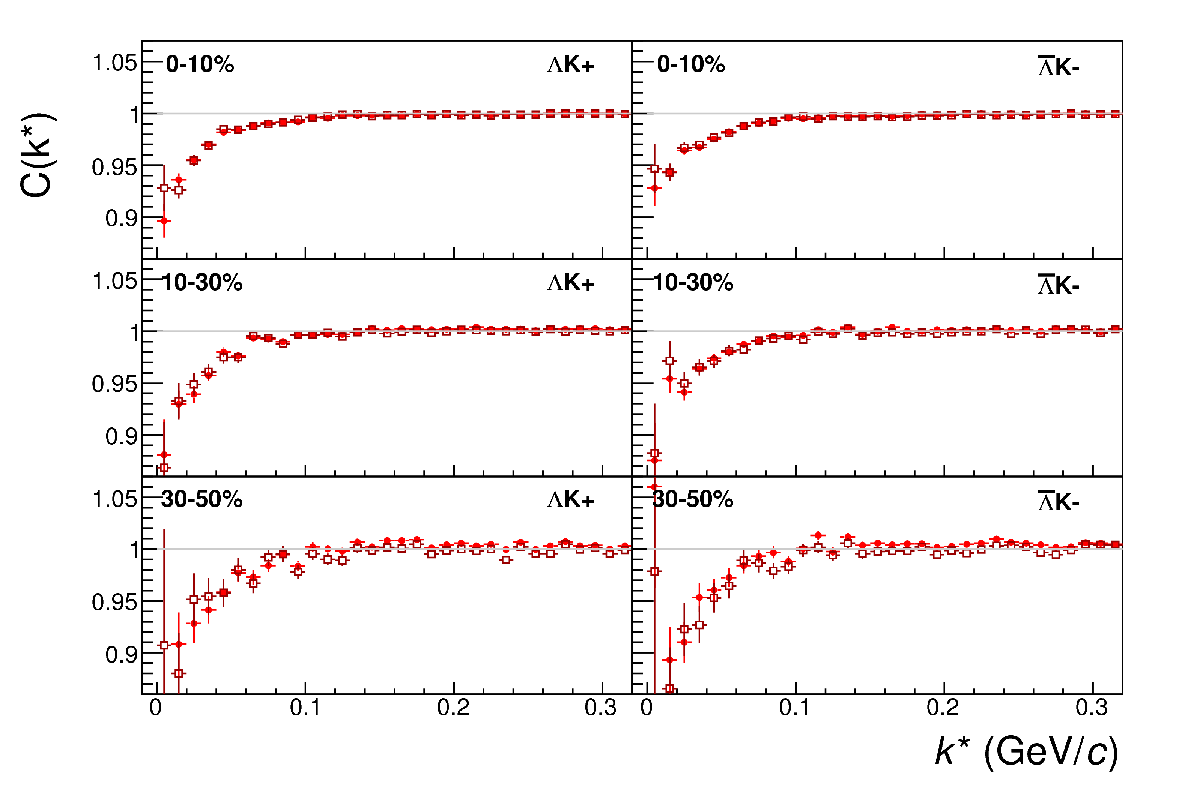
\includegraphics[width=0.49\textwidth]{4_CorrelationFunctions/Figures/WithAdditionalPairCut_20180505/canKStarCfsZoomLamKchPwConj_20180505vs20180505StavCf.pdf}}
  %%----start of second subfigure---
  \subfloat[\LamKchM (left) and \ALamKchP (right) correlations for 0-10\% (top), 10-30\%(middle), and 30-50\%(bottom) centralities.]{
    \label{fig:AllStavCfs:b}
    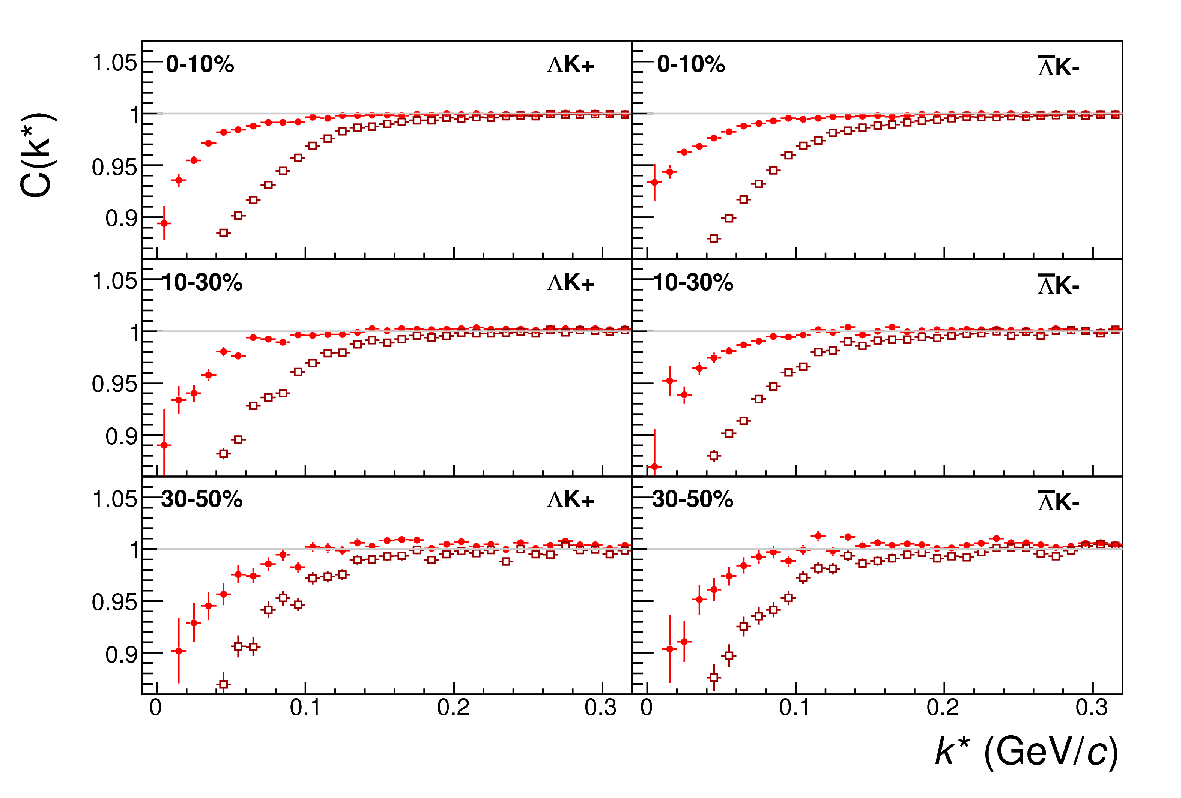
\includegraphics[width=0.49\textwidth]{4_CorrelationFunctions/Figures/WithoutAdditionalPairCut_20180416/canKStarCfsZoomLamKchPwConj_20180416vs20180416StavCf.pdf}}
  \\    
  
  %%----start of third subfigure---  
  \subfloat[\LamKchP (left) and \ALamKchM (right) correlations for 0-10\% (top), 10-30\%(middle), and 30-50\%(bottom) centralities.]{
    \label{fig:AllStavCfs:a}
    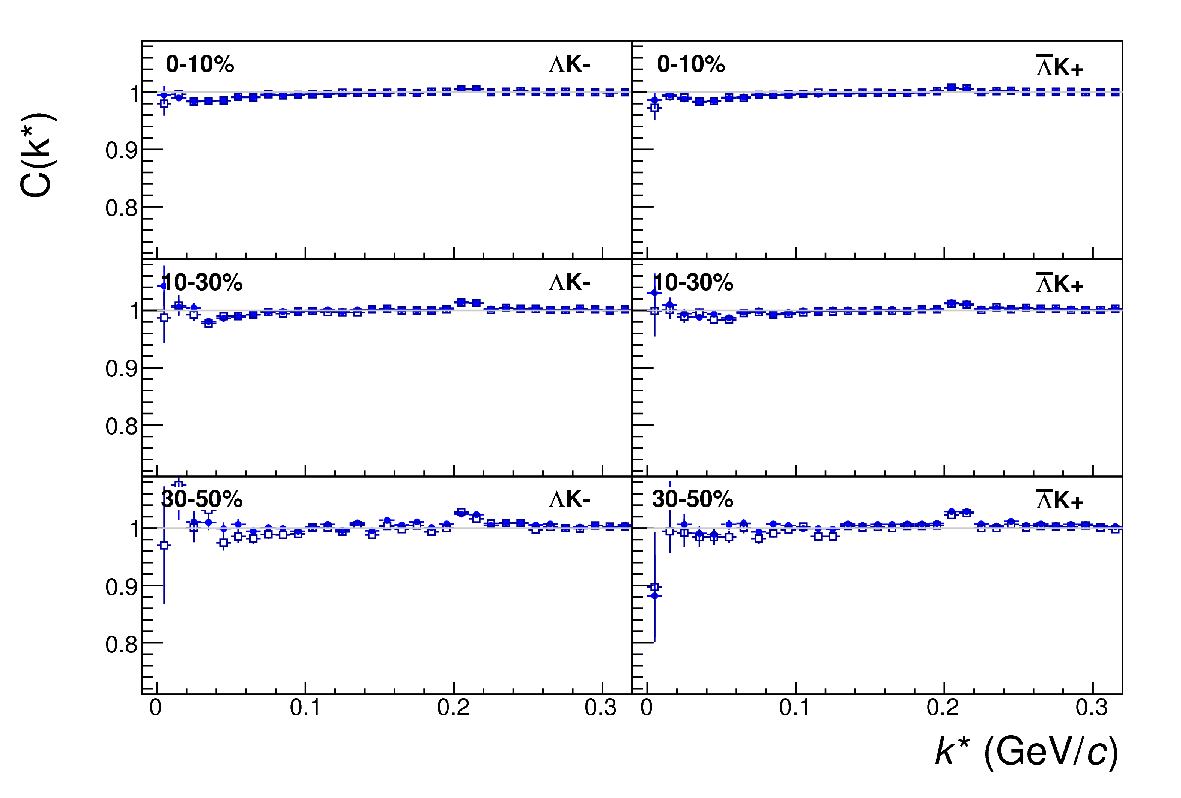
\includegraphics[width=0.49\textwidth]{4_CorrelationFunctions/Figures/WithAdditionalPairCut_20180505/canKStarCfsZoomLamKchMwConj_20180505vs20180505StavCf.pdf}}
  %%----start of fourth subfigure---
  \subfloat[\LamKchM (left) and \ALamKchP (right) correlations for 0-10\% (top), 10-30\%(middle), and 30-50\%(bottom) centralities.]{
    \label{fig:AllStavCfs:b}
    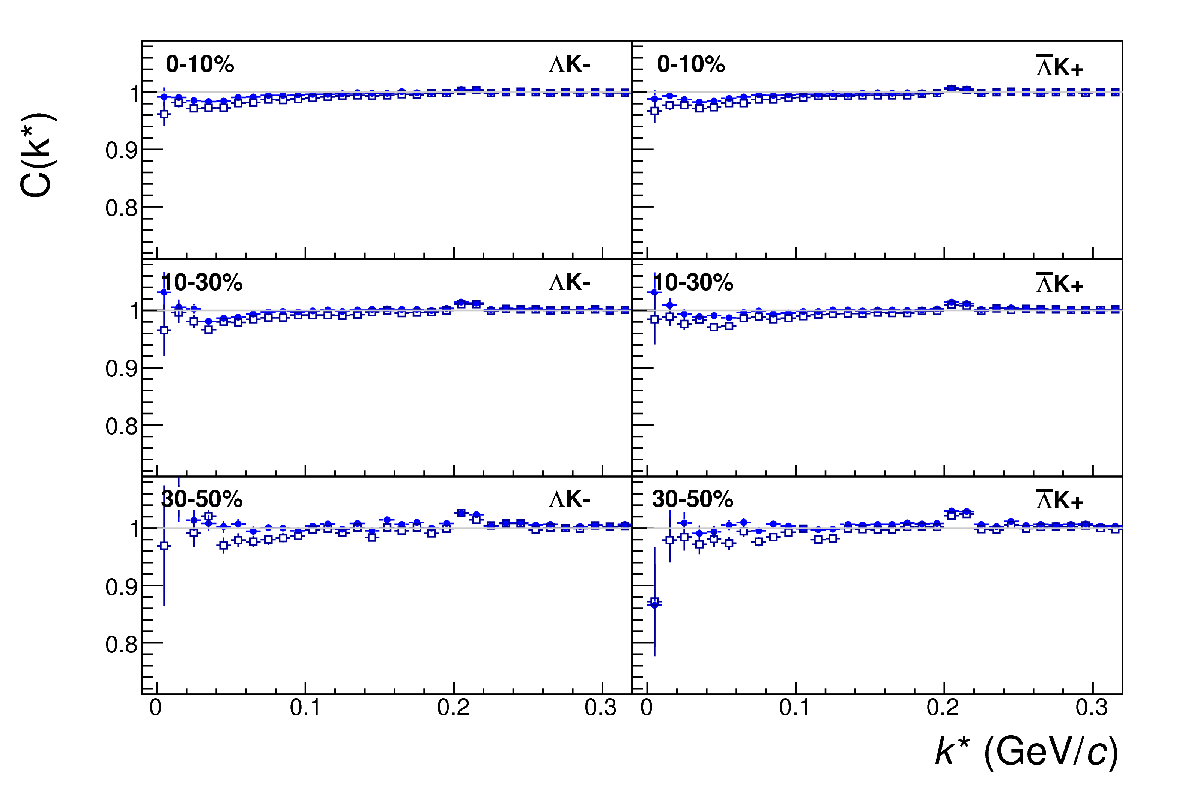
\includegraphics[width=0.49\textwidth]{4_CorrelationFunctions/Figures/WithoutAdditionalPairCut_20180416/canKStarCfsZoomLamKchMwConj_20180416vs20180416StavCf.pdf}}
  \\    
    
  %%----start of fifth subfigure---  
  \subfloat[\LamKchP (left) and \ALamKchM (right) correlations for 0-10\% (top), 10-30\%(middle), and 30-50\%(bottom) centralities.]{
    \label{fig:AllStavCfs:a}
    \includegraphics[width=0.49\textwidth]{4_CorrelationFunctions/Figures/WithAdditionalPairCut_20180505/canKStarCfsZoomLamK0wConj_20180505vs20180505StavCf.pdf}}
  %%----start of sixth subfigure---
  \subfloat[\LamKchM (left) and \ALamKchP (right) correlations for 0-10\% (top), 10-30\%(middle), and 30-50\%(bottom) centralities.]{
    \label{fig:AllStavCfs:b}
    \includegraphics[width=0.49\textwidth]{4_CorrelationFunctions/Figures/WithoutAdditionalPairCut_20180416/canKStarCfsZoomLamK0wConj_20180416vs20180416StavCf.pdf}}
  \\         
    
  %%----overall caption----
  \caption[\LamK Stavinsky Correlation Functions]{\LamK and \ALamAK correlation functions built using the Stavinsky method for 0-10\%, 10-30\%, and 30-50\% centralities.}
  \label{fig:AllStavCfs}
\end{figure}





\end{document}